\section{Observation and Calculation}
	\subsection{Aluminium scatterer}
		\begin{figure}[H]
			\centering
			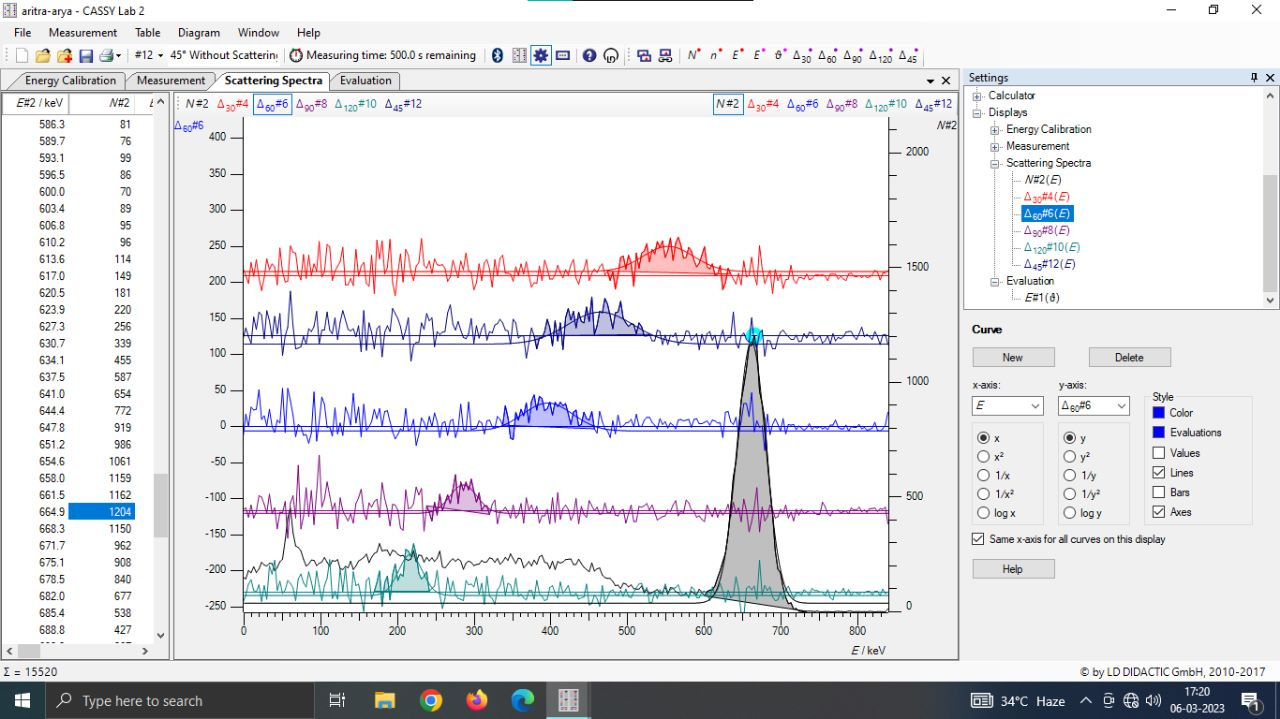
\includegraphics[width=0.8\columnwidth]{images/o_1.png}
			\caption{Measurement spectra}
			\label{graph:1}
		\end{figure}
		\begin{figure}[H]
			\centering
			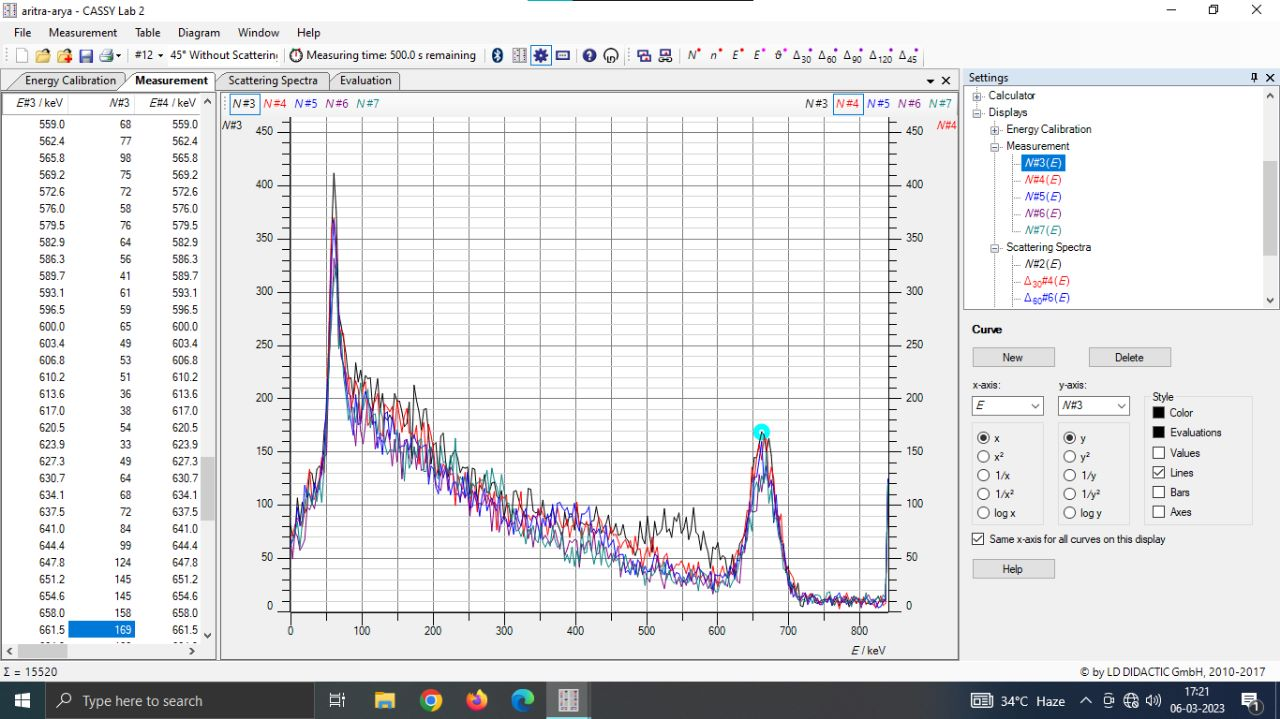
\includegraphics[width=0.8\columnwidth]{images/o_3.png}
			\caption{Scattering spectra}
			\label{graph:2}
		\end{figure}
		\begin{figure}[H]
			\centering
			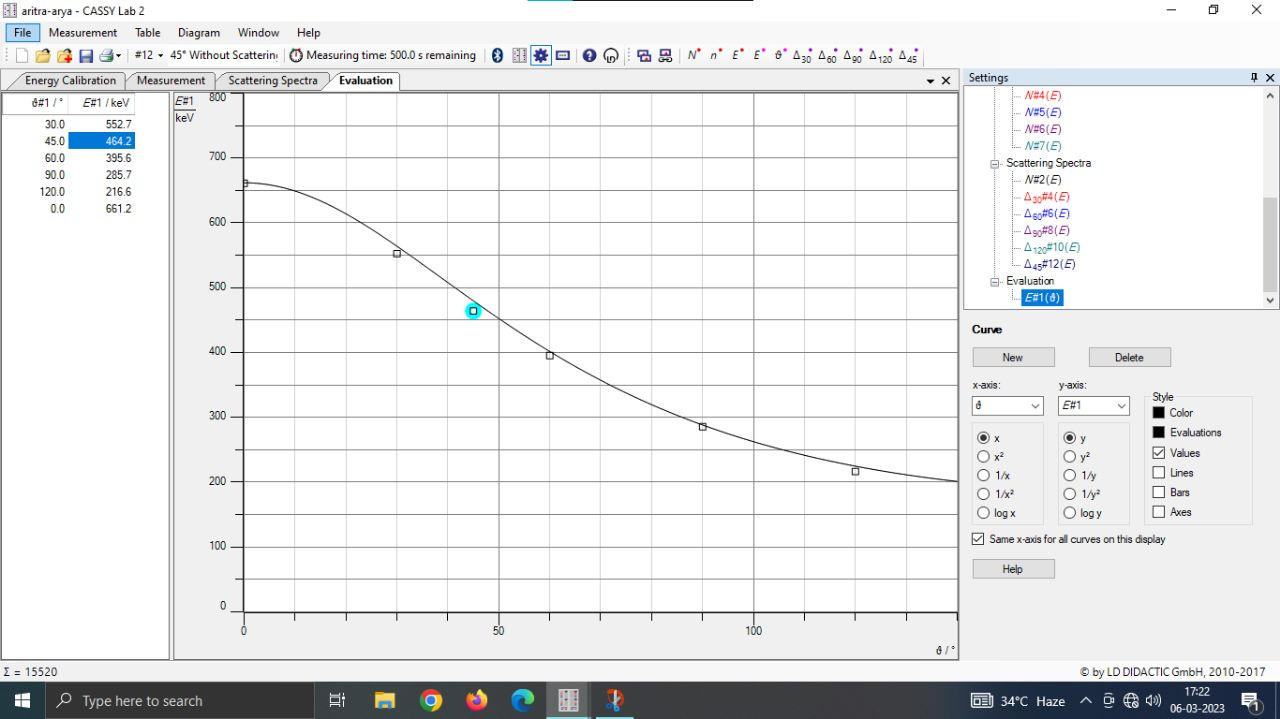
\includegraphics[width=0.8\columnwidth]{images/o_4.png}
			\caption{Energy calibration spectra}
			\label{graph:3}
		\end{figure}

		\begin{table}[H]
    \centering
    \begin{tabular}{|c|c|}
        \hline
        sl no. & background \\ \hline
        1      & 84         \\ \hline
        2      & 60         \\ \hline
        3      & 65         \\ \hline
        4      & 74         \\ \hline
        5      & 69         \\ \hline
        avg    & 70.4       \\ \hline
    \end{tabular}
    \label{tab:1}
    \caption{Background counts for 60s}
\end{table}
		\begin{table}[H]
    \centering
    \begin{tabular}{|c|c|c|}
        \hline
        thickness & count & net count \\ \hline
        0         & 1216  & 204       \\ \hline
        0.6       & 853   & 783       \\ \hline
        0.12      & 706   & 636       \\ \hline
        0.18      & 504   & 434       \\ \hline
        0.24      & 420   & 350       \\ \hline
        0.3       & 311   & 241       \\ \hline
        0.36      & 222   & 152       \\ \hline
        0.42      & 199   & 129       \\ \hline
        0.48      & 168   & 98        \\ \hline
        0.54      & 145   & 75        \\ \hline
    \end{tabular}
    \label{tab:2}
    \caption{$\beta$ praticle counts for  $Tl^{204}$ in aluminium absorber}
\end{table}

		From \hyperref[tab:2]{Table 2} and \hyperref[eq:4]{Equation 4}, we have the calibration factor for aluminum is:
		$$C=2.71\times 10^{32}$$

		By analysing the energy calibration spectra we get $m_e=482.38 KeV$.


	\subsection{Brass scatterer}
		\begin{figure}[H]
			\centering
			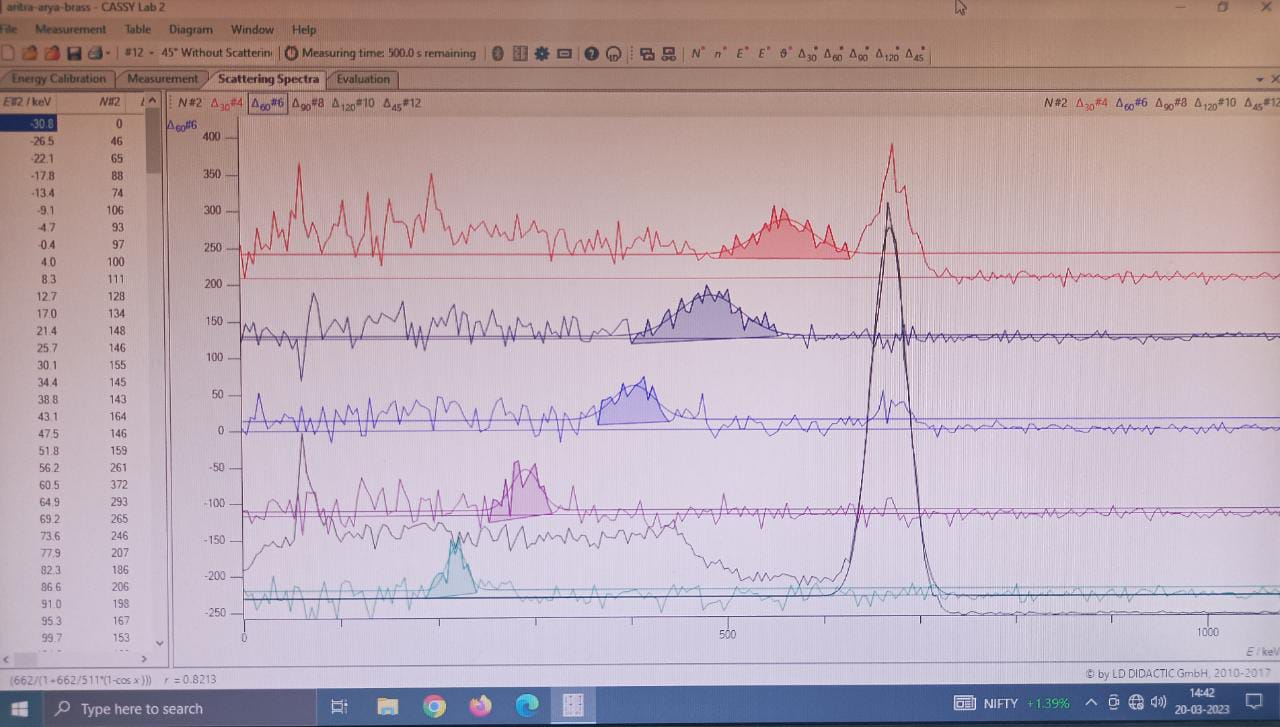
\includegraphics[width=0.75\columnwidth]{images/o_6.png}
			\caption{Measurement spectra}
			\label{graph:4}
		\end{figure}
		\begin{figure}[H]
			\centering
			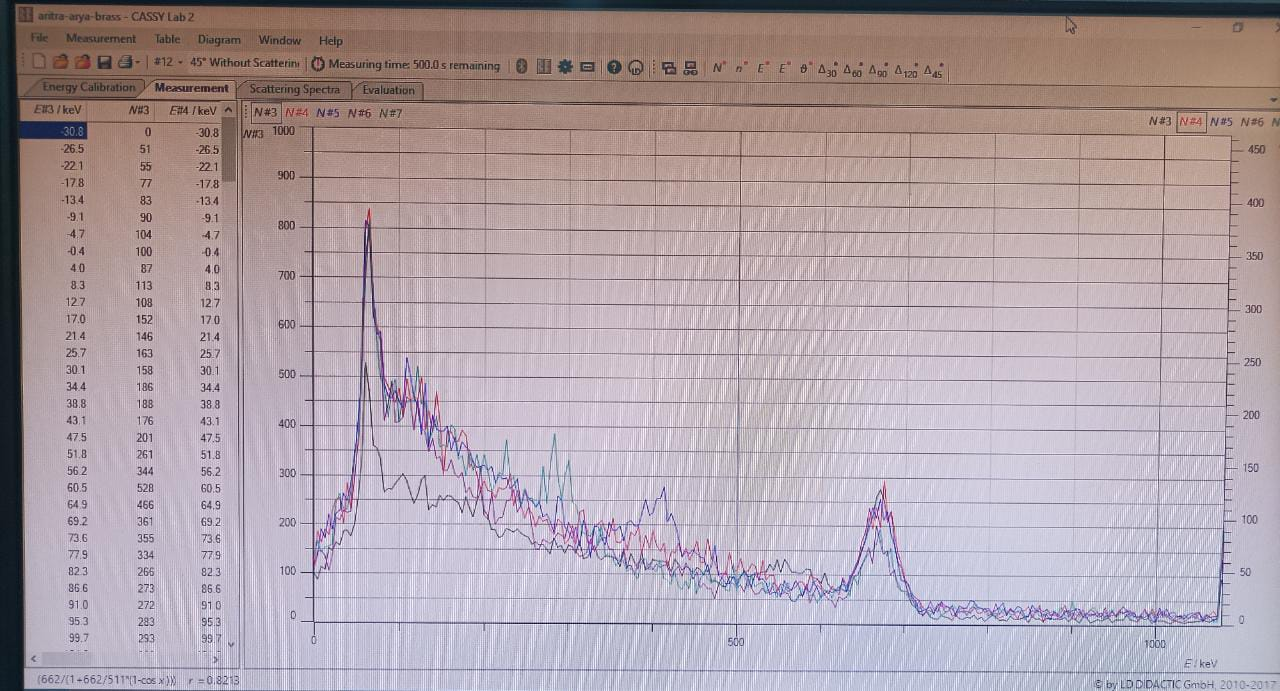
\includegraphics[width=0.75\columnwidth]{images/o_7.png}
			\caption{Scattering spectra}
			\label{graph:5}
		\end{figure}
		\begin{figure}[H]
			\centering
			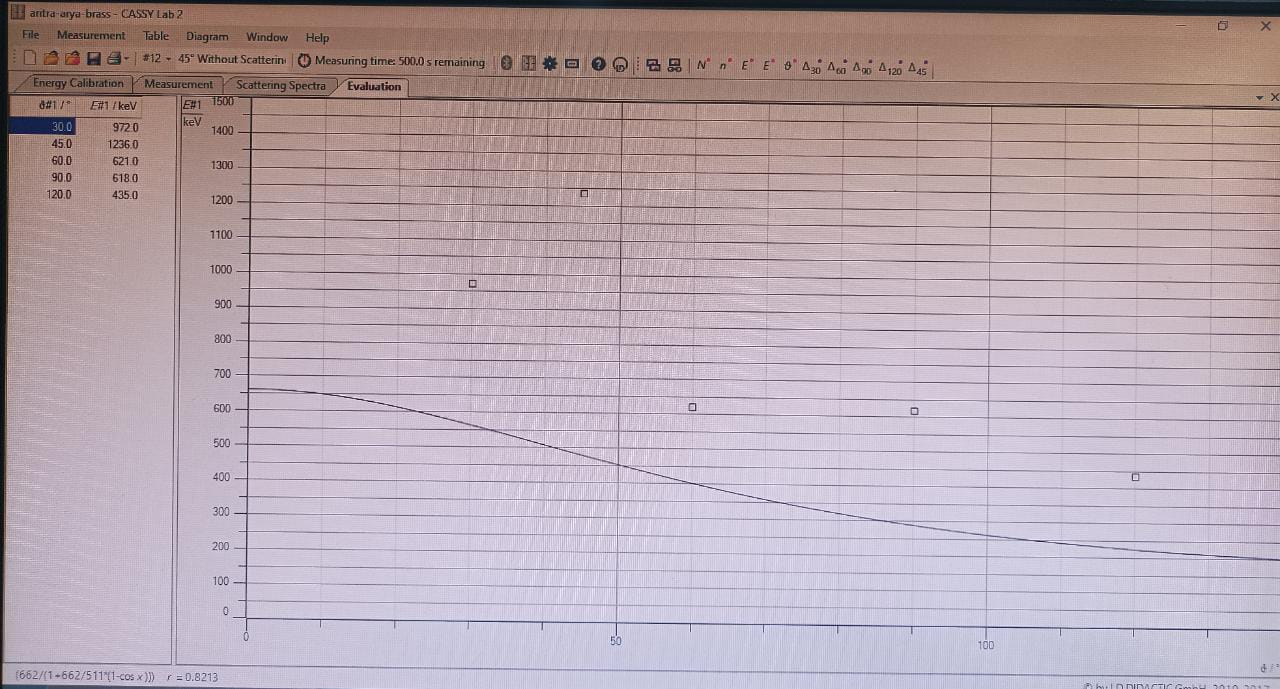
\includegraphics[width=0.75\columnwidth]{images/o_5.png}
			\caption{Energy calibration spectra}
			\label{graph:6}
		\end{figure}

		\begin{table}
    \centering
    \begin{tabular}{|c|c|c|}
        \hline
        angle $\theta$ & change in energy(keV) & change in wavelength($10^{-12}m$) \\ \hline
        30             & 559.4                 & 2.222023597                       \\ \hline
        45             & 481.2                 & 2.58312552                        \\ \hline
        60             & 402.4                 & 3.088966203                       \\ \hline
        90             & 289.8                 & 4.289164941                       \\ \hline
        120            & 218.4                 & 5.691391941                       \\ \hline
    \end{tabular}
    \caption{Change in energy and wavelength as a function of scattering angle for brass}
    \label{tab:3}
\end{table}
		\begin{table}
    \centering
    \begin{tabular}{|c|c|c|}
        \hline
        angle $\theta$ & differential cross-section($10^{-30}m^2$) & relative intensity \\ \hline
        30             & 6.075                                     & 1705               \\ \hline
        45             & 3.348                                     & 1229               \\ \hline
        60             & 2.2                                       & 925                \\ \hline
        90             & 1.3047                                    & 617                \\ \hline
        120            & 0.5581                                    & 550                \\ \hline
    \end{tabular}
    \caption{Evaluation of differential cross-sections and relative intensities for Aluminium}
    \label{tab:4}
\end{table}

		From \hyperref[tab:4]{Table 4} and \hyperref[eq:4]{Equation 4}, we have the calibration factor for brass is:
		
		$$C=5.05\times 10^{32}$$
		
		From energy calibration spectra, we have the rest mass of electron $m_e =419.6Kev$
